%% KOMA-Script Report-Klasse:
\documentclass[12pt,
    abstracton,
	a4paper,
	oneside,
	BCOR10mm,
	pagesize,
	bibliography=totoc,
	listof=totoc
	%draft
	]{scrreprt}

\usepackage[utf8]{inputenc}			% UTF-8 encoding
\usepackage[ngerman]{babel}			% neue deutsche Rechtschreibung
\setcounter{secnumdepth}{4}			% 4 Ebenen bei Nummerierung


%% Header und Footer:
\usepackage[plainheadsepline,plainfootsepline]{scrpage2}
\setheadsepline{0.4pt}
\ihead{\leftmark}\ohead{\pagemark}\chead{}\cfoot{}\ifoot{}\ofoot{}
\pagestyle{scrheadings}
\automark[section]{chapter}


%% Chapter header sinnvoll:
\defpagestyle{myChapterHeader}{
	(0pt,0pt)			% linie oben
	{\pagemark\hfill\leftmark}	% gerade seite
	{\leftmark\hfill\pagemark}	% ungerade seite
	{\leftmark\hfill\pagemark}	% einseitig
	(\textwidth,1pt)		% linie unten
}{%
	(0pt,0pt)			% linie oben
	{}				% gerade seite
	{}				% ungerade seite
	{}				% einseitig
	(0pt,0pt)			% linie unten
}
\renewcommand*{\chapterpagestyle}{myChapterHeader}


%% Seitenränder:
\usepackage[a4paper,left=3.5cm,right=2cm,top=2.5cm,bottom=2.5cm,includeheadfoot]{geometry}


%% Formatierung Schriftarten einstellen:
\usepackage[onehalfspacing]{setspace}		% 1,5facher Zeilenabstand
\usepackage[T1]{fontenc}
\usepackage{lmodern}
\setkomafont{chapter}{\fontsize{20pt}{20pt}\selectfont}
\setkomafont{section}{\fontsize{16pt}{16pt}\selectfont}
\setkomafont{subsection}{\fontsize{14pt}{14pt}\bfseries}
\setkomafont{subsubsection}{\normalsize\mdseries\itshape}
\setkomafont{paragraph}{\normalsize\mdseries}
\setkomafont{subparagraph}{\normalsize\mdseries}


%% nützliche Features:
\usepackage{blindtext}				% lorem ipsum baby!
\usepackage{mdwlist}				% kompaktere Listen mit itemize* und co
\usepackage{graphicx}				% Grafiken
\usepackage{tabularx}				% Tabellen
\usepackage{multirow}				% Mehrzeiliges in Tabellen
\usepackage[table]{xcolor}			% alternierende Farben in Tabellen
\usepackage{rotating}				% Rotieren von Text & co
\usepackage{color}				    % Alles in Bunt und Farbe
\usepackage{multicol}				% multicol halt
\usepackage{amsmath}				% für mathematische Formeln
\usepackage{amsthm}				    % für theoremstyle
\usepackage{amssymb}				% für mathematische Symbole
\usepackage{wrapfig}				% umflossene figures
\usepackage{float}				    % für [h!] bzw. [H] positionierung
\usepackage{scrhack}                % FIX um Warnungen beim listingspaket zu umgehen
\usepackage{pdfpages}

%% Glossar
\usepackage[ngerman]{translator}
\usepackage[style=super,nonumberlist, nowarn]{glossaries}
\makeglossaries


%% Abkürzungsverzeichnis
\usepackage[german]{nomencl}
\renewcommand{\nomname}{Glossar und Abkürzungsverzeichnis}
\renewcommand{\nomlabel}[1]{\hfil \textbf{#1}\hfil}
\makenomenclature


%% Literaturverzeichnis
\usepackage[round]{natbib}
\usepackage{bibgerm}


%% Quelltexte:
\usepackage{listings}
\lstset{ %
	basicstyle=\scriptsize, 		% the size of the fonts that are used for the code
	numbers=left,				% where to put the line-numbers
	numberstyle=\footnotesize,		% the size of the fonts that are used for the line-numbers
	backgroundcolor=\color{white},		% choose the background color. You must add \usepackage{color}
	commentstyle=\color{gray},
	xleftmargin=1.5em,
	xrightmargin=1em,
	frame=tb,				% adds a frame around the code
	tabsize=2,				% sets default tabsize to 2 spaces
	captionpos=b,				% sets the caption-position to top or bottom
	breaklines=true,			% sets automatic line breaking
	breakatwhitespace=false			% sets if automatic breaks should only happen at whitespace	
}
\renewcommand*{\lstlistingname}{Quelltext}
\renewcommand*{\lstlistlistingname}{Quelltextverzeichnis}


%% Tikz für (komplizierte) bunte Bildchen:
\usepackage{tikz}
\usetikzlibrary{positioning,mindmap,shapes,shapes.multipart,shadows,arrows,patterns,topaths}

\definecolor{gelb}{HTML}{FFFCCC}
\definecolor{gruen}{HTML}{CFFFCC}
\definecolor{blau}{HTML}{CCE9FF}
\definecolor{dunkelblau}{HTML}{99b7EE}
\definecolor{rot}{HTML}{FFA8A8}
\definecolor{orange}{HTML}{FFD28F}


%% PDF Optionen (verweise und co):
\usepackage[pdftex, raiselinks, pdfpagelabels, plainpages=false, hypertexnames=false,
            pdfborder=false]{hyperref}
\pdfcompresslevel=0
\hypersetup{
    pdfauthor = {Marc Ludwig, Matthias Springstein},
    pdftitle = {Beleg zum Semesterprojekt - Distanzmessung mittels Ultraschall},
    pdfsubject = {Beleg},
    pdfkeywords = {Ultraschall, ultrasonic, range},
    pdfcreator = {LaTeX with hyperref package}
}

%% Fix wegen langen url's i mAnhang
\usepackage{etoolbox}
\apptocmd{\thebibliography}{\raggedright}{}{}

%% Eigene Kommandos (Zitate, Verweise, Theoreme):
\newcommand{\zitat}[2][]{(\citealt[#1]{#2})}
\newcommand{\zitatalt}[2][]{\citet[#1]{#2}}
\newcommand{\zitatsiehe}[2][]{(siehe \citealt[#1]{#2})}
\newcommand{\zitatnach}[2][]{(nach \citealt[#1]{#2})}

%% nameref umbiegen für Verweise auf andere Kapitel :
\newcommand{\siehe}[1]{\ref{#1} \emph{\nameref{#1}} [S. \pageref{#1}]}

%% eigenen Theoremstil für Definitionen:
\newtheoremstyle{mystyle}			% name of the style to be used
{}						% measure of space to leave above the theorem. E.g.: 3pt
{}						% measure of space to leave below the theorem. E.g.: 3pt
{\itshape}					% name of font to use in the body of the theorem
{}						% measure of space to indent
{\bfseries}					% name of head font
{:}						% punctuation between head and body
{3pt}						% space after theorem head
{}						% Manually specify head

\theoremstyle{mystyle}
\newtheorem{definition}{Definition}


%% Workarounds und fixes:

%% Umbruch in Texttt enviroment mist
\newcommand{\breaktt}[1]{\texttt{\hyphenchar\font45\relax #1}}

%% Ermöglicht das Einfügen von *.svg Grafiken
\newcommand{\executeiffilenewer}[3]{%
\ifnum\pdfstrcmp{\pdffilemoddate{#1}}%
{\pdffilemoddate{#2}}>0%
{\immediate\write18{#3}}\fi%
}
% includesvg[scale]{file}
\newcommand{\includesvg}[2][1]{%
  \executeiffilenewer{#1.svg}{#1.pdf}{%
  /usr/bin/inkscape -z -D --file="#2.svg" --export-pdf="#2.pdf" --export-latex}%
  \scalebox{#1}{\input{#2.tex}}%
}

%% viel zu großen vspace des chapters beseitigen
\renewcommand*{\chapterheadstartvskip}{\vspace*{-\topskip}}

%% fix für merkwürde "lücken" bei doppelseitigem layout:
\renewcommand{\pagebreak}{\vfill\newpage}

\begin {document}
	%% Titelseite
	\pdfbookmark[1]{Titelseite}{titlepage}
	\linespread{1.05}\selectfont % 1,5-zeilig aus

\titlehead{
	\centering
	
\includegraphics[width=\textwidth]{img/unilogo.png}\\
	\vspace{1em}
}

\subject{Beleg}
\title{Numerische Mathematik - Problem2: schlecht konditioniertes LGS}
\subtitle{\vspace{2cm}}

\author{\textbf{\parbox{0.9\textwidth}{
    \centering
    Marc Ludwig\\
    Marvin Hohlfeld\\
    Matthias Bukovsky\\
    Matthias Springstein}}}
\date{\normalsize Jena, \today}

\publishers{\large 

\begin{tabular}{rl}
Betreuer:& Prof. P. Wilde
\end{tabular}
}

\maketitle

	%% Inhaltsverzeichnis
	\newpage
	\thispagestyle{empty}
	\null

	\pagenumbering{Roman}
	\clearpage\setcounter{page}{1}

	\pdfbookmark[1]{Inhaltsverzeichnis}{tableofcontents}
	\tableofcontents
	\pagebreak
	
	\newpage
	\thispagestyle{empty}
	\null	

    \renewcommand{\abstractname}{Abstract}    
    \begin{abstract}
      
    \end{abstract}

    %% Eigentlicher Inhalt
    \pagenumbering{arabic}
    \clearpage\setcounter{page}{1}

	\chapter{Entwickle die Funktion \emph{f} aus obigem Problem in eine Taylorreihe}

\section{Die Taylorreihe}
In der Analysis verwendet man Taylorreihen (auch Taylor-Entwicklungen, nach dem Mathematiker Brook
Taylor\footnote{Brook Taylor (* 18. August 1685 in Edmonton, Middlesex; † 29. Dezember 1731 in
Somerset House, London) war ein britischer Mathematiker. Nach ihm wurde u.a. die Taylorreihe
benannt.}), um Funktionen in der Umgebung bestimmter Punkte durch Potenzreihen darzustellen
(Reihenentwicklung). So kann ein komplizierter analytischer Ausdruck durch eine nach wenigen
Gliedern abgebrochene Taylorreihe (oftmals gut) angenähert werden, z.B. in der Physik oder bei der
Ausgleichung geodätischer Netze: So ist die oft verwendete Kleinwinkelnäherung des Sinus eine nach
dem ersten Glied abgebrochene Taylorreihe dieser Funktion.

\section{Definition}
Sei \( I \subset \mathrm{R} \) ein offenes Intervall, \( f \colon I \rightarrow \mathrm{R} \) eine
unendlich oft differenzierbare Funktion und \(a\) ein Element von \(I\). Dann heißt die unendliche
Reihe
\begin{align}
        \label{eq:taylorreihe1}
P_f(x)  & = f(a) + \frac{f'(a)}{1!} (x-a) + \frac{f''(a)}{2!} (x-a)^2 + \dotsb +
            \frac{f^{(n)}(a)}{n!} (x-a)^n + \dotsb\\
        \label{eq:taylorreihe2}
        & = \sum_{n=0}^\infty \frac{f^{(n)}(a)}{n!} (x-a)^n
\end{align}
die Taylor-Reihe von f mit Entwicklungsstelle a.

Hierbei bezeichnet
\begin{itemize}
    \item   \(n!\) die Fakultät \(n! = 1 \cdot 2 \cdot \dots \cdot n\) und
    \item   \(f^{(n)}(a)\) die n-te Ableitung von \(f\) an der Stelle a, wobei man \(f^{(0)} := f\)
            setzt.
\end{itemize}

\section{Eigenschaften}
Die Taylorreihe \(P_f(x)\) zur Funktion \(f(x)\) ist eine Potenzreihe \(P\) in \(x\). Im Fall einer
analytischen Funktion \(f\) hat die Taylor-Reihe in jedem Punkt \(a\) einen positiven
Konvergenzradius \(r\) und stimmt in ihrem Konvergenzbereich mit \(f\) überein, d.h. es gibt ein
\(r>0\), sodass für \(|x-a|<r\) gilt
\begin{equation}
    P_f(x) = \sum_{n=0}^\infty a_n (x-a)^n = f(x)
\end{equation}.
Außerdem stimmen die Ableitungen der Reihe im Entwicklungspunkt \(a\) mit den tatsächlichen
Ableitungswerten überein:
\begin{equation}
    P_f^{(k)}(a) = f^{(k)}(a)
\end{equation}
.
    
\section{Konstruktion}
Damit die Ableitungen der Reihe im Entwicklungspunkt \(a\) mit den tatsächlichen Ableitungswerten
übereinstimmen, sind die Koeffizienten \(a_n\) der Taylorreihe wie folgt konstruiert:
\begin{equation}
    \label{eq:konstruktion}
    a_n = \frac{f^{(n)}(a)}{n!} \Rightarrow P_f(x) = \sum_{n=0}^\infty \frac{f^{(n)}(a)}{n!} (x-a)^n
\end{equation}
.

\section{Entwicklung von \emph{f(x)} in eine Tylor Reihe}
Bei gegebener Funktion
\begin{equation}
    f\left(x\right) = \frac{1}{1+x}
\end{equation}
und den Gleichungen \ref{eq:taylorreihe1} und \ref{eq:taylorreihe2} folgt für deren Ableitungen
\begin{align}
    f'\left(x\right)    &= -\frac{1}{\left(1+x\right)^2} \\
    f''\left(x\right)   &=  \frac{2\left(1+x\right)}{\left(1+x\right)^4}
                         =  \frac{2}{\left(1+x\right)^3} \\
    f'''\left(x\right)  &=  \frac{2\left(1+x\right)^4 -8\left(1+x\right)\left(1+x\right)^3}
                            {\left(1+x\right)^8}
                         =  -\frac{6}{\left(1+x\right)^4}
\end{align}
Hieraus läßt sich folgende Bildungsvorschrifft für eine beliebige Ableitung bestimmen
\begin{equation}
    f^n\left(x\right) = \left(-1\right)^n \frac{n!}{\left(1+x\right)^{n+1}}
\end{equation}
hieraus folgt nach Gleichung \ref{eq:konstruktion}
\begin{align}
    f\left(x\right)  =  P_f\left(x\right) 
                    &= \sum_{n=0}^{\infty} \left(-1\right)^n
                        \frac{n!}{n!\left(1+a\right)^{n+1}}\left(x-a\right)^n\\
                    &=  \sum_{n=0}^{\infty} \left(-1\right)^n
                        \frac{\left(x-a\right)^n}{\left(1+a\right)^{n+1}}
\end{align}
	\chapter{Nachweis der hermiteschen Form von \emph{H}}
Eine hermitesche Matrix oder selbstadjungierte Matrix wird im mathematischen Teilgebiet der Linearen
Algebra untersucht. Es handelt sich um eine spezielle Art von quadratischen Matrizen. Benannt sind
diese nach dem Mathematiker Charles Hermite\footnote{Charles Hermite (* 24. Dezember 1822 in Dieuze
(Lothringen); † 14. Januar 1901 in Paris) war ein französischer Mathematiker.}.

\section{Definition - hermitesch}
Eine \(n \times n\)-Matrix \(A\) mit Einträgen in \(\mathrm{C}\) heißt hermitesch, wenn sie mit
ihrer (hermitesch) Adjungierten \(A^*\), also der transponierten und komplex konjugierten Matrix
übereinstimmt. Das heißt, wenn
\begin{equation}
    A = A^* = \overline A^{\mathrm T} = \overline{A^{\mathrm T}}
\end{equation}
gilt.

Für die adjungierte Matrix finden sich auch die Bezeichnungen \(A^\dagger\) und \(A^{\mathrm H}\).
Die Schreibweise \(A^*\) wird auch für die komplex konjugierte Matrix verwendet.

Für die Einträge einer hermiteschen Matrix gilt also:
\begin{equation}
\label{eq:elements}
    a_{jk} = \overline{a_{kj}}
\end{equation}
Anders formuliert ist eine Matrix A genau dann hermitesch, wenn ihre Transponierte gleich ihrer
komplex Konjugierten ist, d.h. \(A^{\mathrm T} = \overline A\).

\subsection{direkte Folgen aus der Definition}
\begin{itemize}
  \label{item:hermSym}
  \item Der Realteil einer hermiteschen Matrix ist symmetrisch, \(\mathrm{Re}(a_{jk}) =
        \mathrm{Re}(a_{kj})\), der Imaginärteil ist schiefsymmetrisch, \(\mathrm{Im}(a_{jk}) =
        -\mathrm{Im}(a_{kj})\).
  \item Ist \(A\) hermitesch, dann ist \(iA\) schiefhermitesch.
  \item Die Hauptdiagonalelemente einer hermiteschen Matrix sind reell.  
  \item Für reelle Matrizen fallen die Begriffe hermitesch und symmetrisch zusammen.
  \item Hermitesche Matrizen sind normal, d. h \(A^* \cdot A = A\cdot A^*\)
\end{itemize}

\section{Mathematischer Beweis für die gegebene Matrize 'H'}
Mit der gegebenen Bildungsvorschrifft
\begin{equation}
    H := \left(\frac{1}{j+k+1}\right)_{j,k=0}^{n}
\end{equation}
Gleichung \ref{eq:elements} und den Aussagen aus \ref{item:hermSym} folgt, dass für \(H\) der
folgende Zusammenhang gillt:
\begin{align}
                                           H &= H^{\mathrm T} \\
                                     H_{j,k} &= H_{k,j}       \\
    \left(\frac{1}{j+k+1}\right)_{j,k=0}^{n} &= \left(\frac{1}{j+k+1}\right)_{k,j=0}^{n}
\end{align}
	\chapter{Eigenwerte und Kondition von H}
Die Erstellung der Matrix \(H\) wird durch ein Octave-Script\footnote{GNU Octave ist eine freie
Software zur numerischen Lösung mathematischer Probleme, wie zum Beispiel Matrizenrechnung, Lösen
von (Differential-)Gleichungssystemen, Integration etc. Berechnungen können in Octave mit einer
Skriptsprache durchgeführt werden, die weitgehend zu dem proprietären MATLAB kompatibel ist.}
organisiert. Siehe hierzu \ref{code:foo} und \ref{code:numa}.

Die berechneten Daten werden in zwei Dateien geschrieben,
\lstset{language=Octave, inputencoding=utf8, literate={Ö}{{\"O}}1 {Ä}{{\"A}}1 {Ü}{{\"U}}1
{ß}{{\ss}}2 {ü}{{\"u}}1 {ä}{{\"a}}1 {ö}{{\"o}}1}
\begin{lstlisting}
    # öffnen und schreiben in eine Datei
    # mögliche Modi: r-read, w-write, a-append
    fileId = fopen ('fileName','mode');
    # do something
        ...
    # done!
    # schließen der Datei nicht vergessen
    fclose (fileId);
\end{lstlisting}
um sie später mit einem externen Programm (z.B. gnuplot) weiter verarbeiten zu können. Ihnen sind
die Werte in Tabelle \ref{tab:task3} entnommen.

\vspace{1em}
\centering    
\begin{table}[htbp]
\tiny
\caption{Eigenwerte \& Konditionen für 3..10xn Matrizen \label{tab:task3}}         
\begin{tabularx}{\textwidth}{|c|X|X|X|X|X|X|X|X|X|X|X|}
    \hline    
    N &&&&&&&&&&& Kond.\\\hline
    3 & 0.00268 & 0.12232 & 1.40831 &&&&&&&& 524.06\\\hline
    4 & 9.6702 e-05 & 6.7383 e-03 & 1.6914 e-01 & 1.5002 e+00 &&&&&&& 1.5514 e+04\\\hline
    5 & 3.2879 e-06 & 3.0590 e-04 & 1.1407 e-02 & 2.0853 e-01 & 1.5671 e+00 &&&&&& 4.7661 e+05\\\hline
    6 & 1.0828 e-07 & 1.2571 e-05 & 6.1575 e-04 & 1.6322 e-02 & 2.4236 e-01 & 1.6189 e+00 &&&&& 1.4951 e+07\\\hline
    7 & 3.4939 e-09 & 4.8568 e-07 & 2.9386 e-05 & 1.0086 e-03 & 2.1290 e-02 & 2.7192 e-01 & 1.6609 e+00 &&&& 4.7537 e+08\\\hline
    8 & 1.1115 e-10 & 1.7989 e-08 & 1.2943 e-06 & 5.4369 e-05 & 1.4677 e-03 & 2.6213 e-02 & 2.9813 e-01 & 1.6959 e+00 &&& 1.5258 e+10\\\hline
    9 & 3.4998 e-12 & 6.4609 e-10 & 5.3856 e-08 & 2.6730 e-06 & 8.7581 e-05 & 1.9789 e-03 & 3.1039 e-02 & 3.2163 e-01 & 1.7259 e+00 && 4.9315 e+11\\\hline
    10& 1.0931 e-13 & 2.2667 e-11 & 2.1474 e-09 & 1.2290 e-07 & 4.7297 e-06 & 1.2875 e-04 & 2.5309 e-03 & 3.5742 e-02 & 3.4293 e-01 & 1.7519 e+00 & 1.6025 e+13\\\hline
\end{tabularx}
\end{table}
	\chapter{Numerische Lösung des LGS für eine fünfstellige Genauigkeit}
Falls H eine \(n \times n\)-Matrix ist, wird von Octave Gaußelimination \footnote{Johann Carl
Friedrich Gauß (latinisiert Carolus Fridericus Gauss; * 30. April 1777 in Braunschweig; † 23.
Februar 1855 in Göttingen) war ein deutscher Mathematiker, Astronom, Geodät und Physiker mit einem
breit gefächerten Feld an Interessen.} verwendet, sonst wird via QR-Zerlegung eine Lösung im Sinne
der kleinsten Fehlerquadrate berechnet. Ist A schlecht konditioniert oder singulär, wird eine
Warnung ausgegeben. Um zu zeigen, dass das Eliminationsverfahren nach Gauß ungeeignet ist haben wir
hierführ eine eigene Funktion gechrieben, welche im Listing \ref{code:gauss} zu sehen ist.

\lstset{label=code:gauss, caption=Gauß-Eliminationsverfahren als Matlab-/Octavescript}
\lstinputlisting{../src/gaussElim.m}
	\chapter{Visualisierung der Koeffezienten sowie des Taylorpolynoms}

\begin{figure}[H]
    \vspace{-1em}
    \begin{center}
        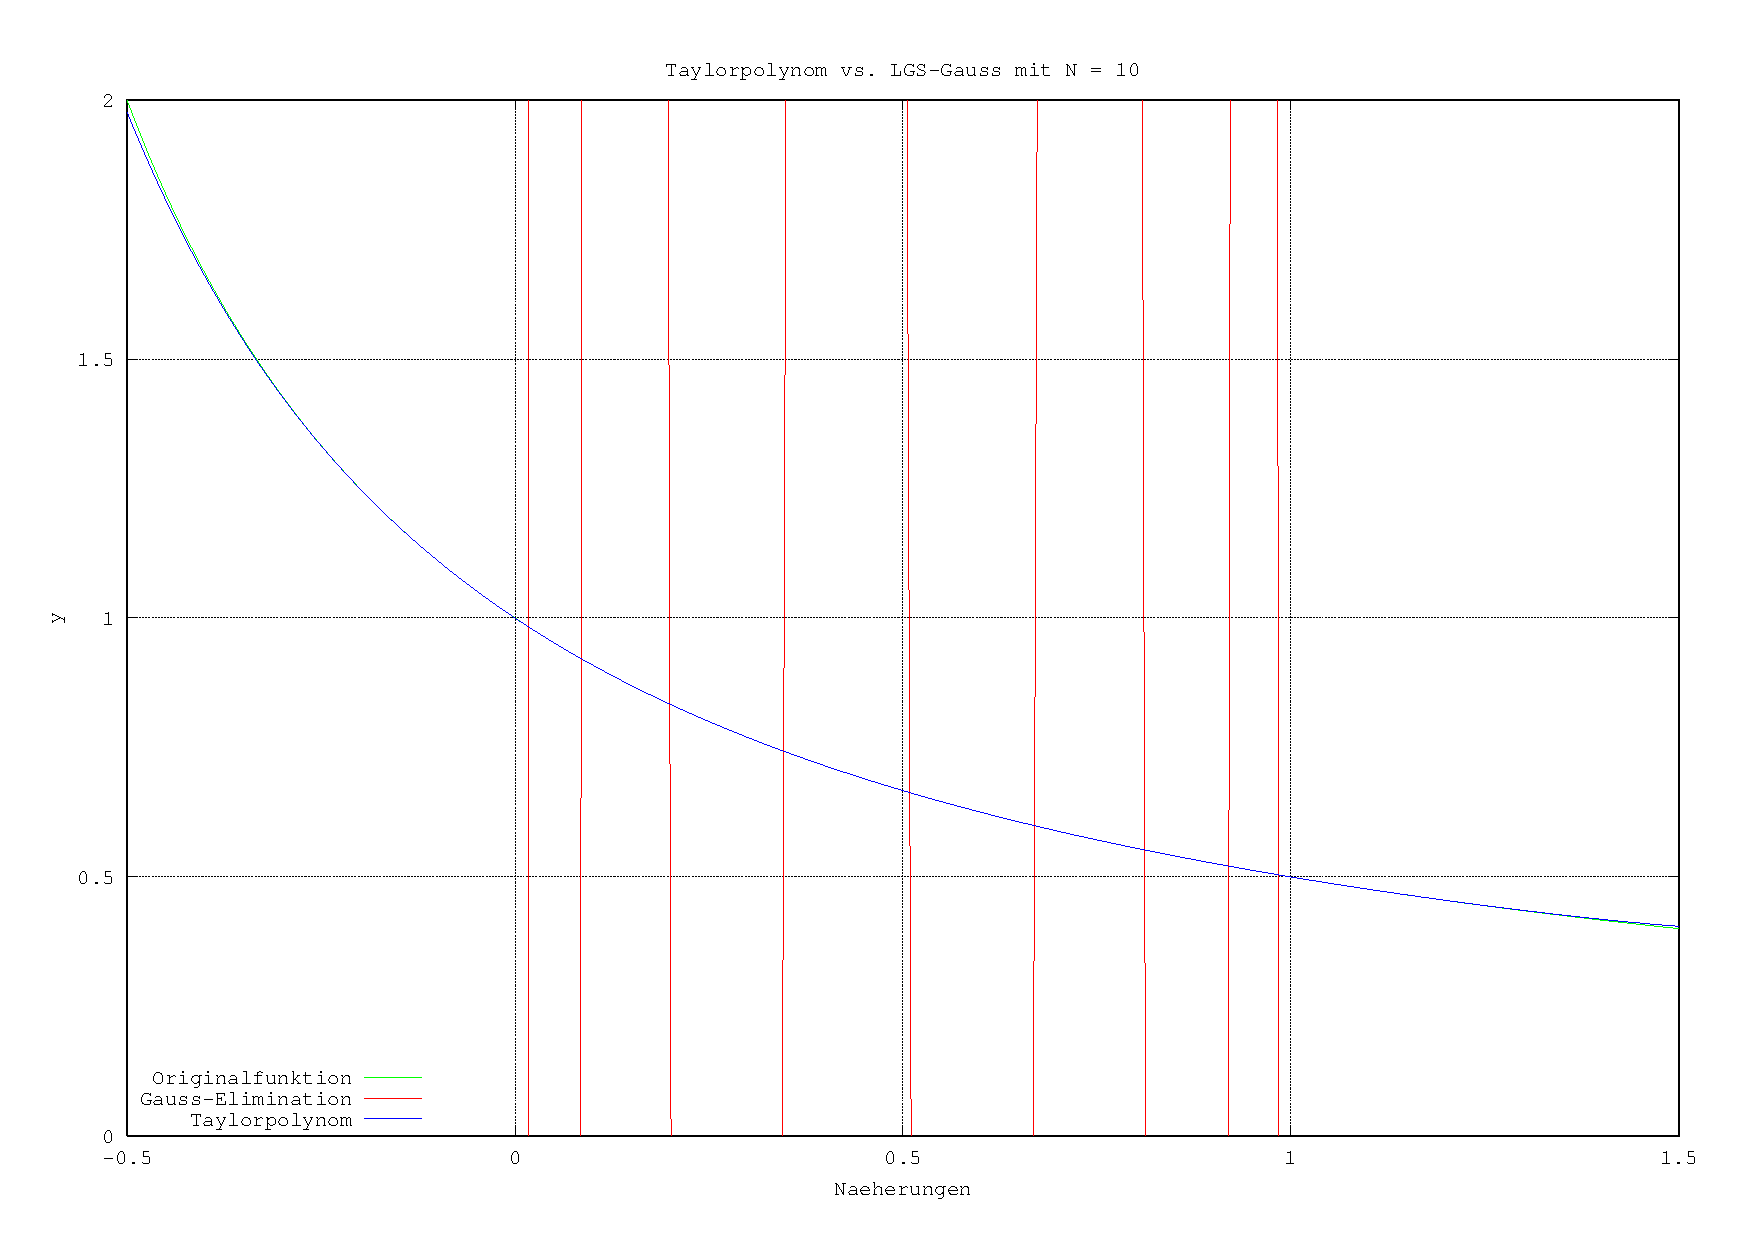
\includegraphics[width=\textwidth]{img/aufgabe5.pdf}
    \end{center}
    \vspace{-1em}
    \caption{Plot des Taylorpolynoms vs. Gauss-Elimination}
    \label{fig:TaylorVsGauss}
\end{figure}
	%% ...

	%% Beginn vom Anhang
	\appendix
	%\pagenumbering{romanian}
	%\clearpage\setcounter{page}{2}

	%% Glossar
	%\nomenclature{Begriff}{Erklärung des Begriffs}

\cleardoublepage% or \clearpage
\markboth{\nomname}{\nomname}

\printnomenclature
\addcontentsline{toc}{chapter}{Glossar und Abkürzungsverzeichnis}


	%% Verzeichnisse
	\newpage
	\listoffigures
 	% \listoftables
	\lstlistoflistings

	%% Literaturverzeichnis
	%\newpage
	%\bibliographystyle{gerapali}
	%\bibliography{quellen}
	%\nocite{*}

	%% sonstiger Anhang:
	\chapter{Anhang}
%-------------------------------------------------------------------------------------------------%
% - Quelltexte - %
%-------------------------------------------------------------------------------------------------%
\section{Quelltexte}
\lstset{language=Octave, inputencoding=utf8, literate={Ö}{{\"O}}1 {Ä}{{\"A}}1 {Ü}{{\"U}}1
{ß}{{\ss}}2 {ü}{{\"u}}1 {ä}{{\"a}}1 {ö}{{\"o}}1}

\lstset{label=code:foo, caption=Foo}
\lstinputlisting{../src/foo.m}

\lstset{label=code:numa, caption=Berechnungen für eine nxn Matrize}
\lstinputlisting{../src/numa.m}

% \lstset{label=code:headerglobal, caption=Globaler Header}
% \lstinputlisting{code/global.h}

\end{document}